

For offline analysis and reconstruction of telescope test beam data the EUTelescope software package~\cite{ref:eutelwebsite}
 is available and features close integration of the EUDAQ software framework described in section~\ref{sec:eudaq}.
EUTelescope builds on the ILCSoft framework~\cite{ref:eudetmemo_2009_12} which provides the basic building blocks for offline analysis such as a generic data model (Linear Collider I/O, LCIO),
a geometry description language (GEAR) and the central event processor (Marlin).

%\cite{EUDET-2008-48}.
Marlin allows for modular composition of analysis chains for various applications. Every task is implemented as an independent processor which is called by Marlin for every event. 
Each processor exposes a set of parameters to the user which can be configured and loaded at runtime via so-called steering files in XML format.
This way the Marlin/Processor architecture gives maximum flexibility to the user.

EUTelescope provides several processors for Marlin, implementing algorithms necessary for a full track reconstruction and data analysis of test beam experiments. 
Figure~\ref{fig:offline:strategy} shows the analysis strategy of the framework starting from the recorded detector response to the final reconstructed particle tracks. 
%An overview of the processor range provided by EUTelescope is given in \cite{EUDET-2007-20}.
At low-energy beam lines such as the DESY-II test beam facility multiple scattering is an important contribution to the overall track resolution uncertainty,
 especially in measurements with non-negligible DUT material budget, cf.\ section~\ref{sec:multiplescattering}.
Therefore EUTelescope provides processors implementing advanced algorithms for tracking such as Deterministic Annealing Filter (DAF)~\cite{ref:daffitter}
 or GBL which account for scattering in all material present in the beam.
For high-energy beam lines a simple straight line fit provides maximum performance.
In addition, precise offline detector alignment can be performed by minimising track residuals using the EUTelescope alignment processor which implements the Millepede-II algorithm~\cite{Blobel-2006}.

EUTelescope comes with its own job submission framework jobsub that allows to run analysis jobs on local machines or to submit them to larger computing clusters such as NAF for bulk reconstruction.
Using its flexible configuration file concept and the global run database storing user defined variables,
 jobsub eases the implementation of per-run variables for reconstruction such as beam energy or detector alignment.

\begin{figure}[tbp]
  \center
  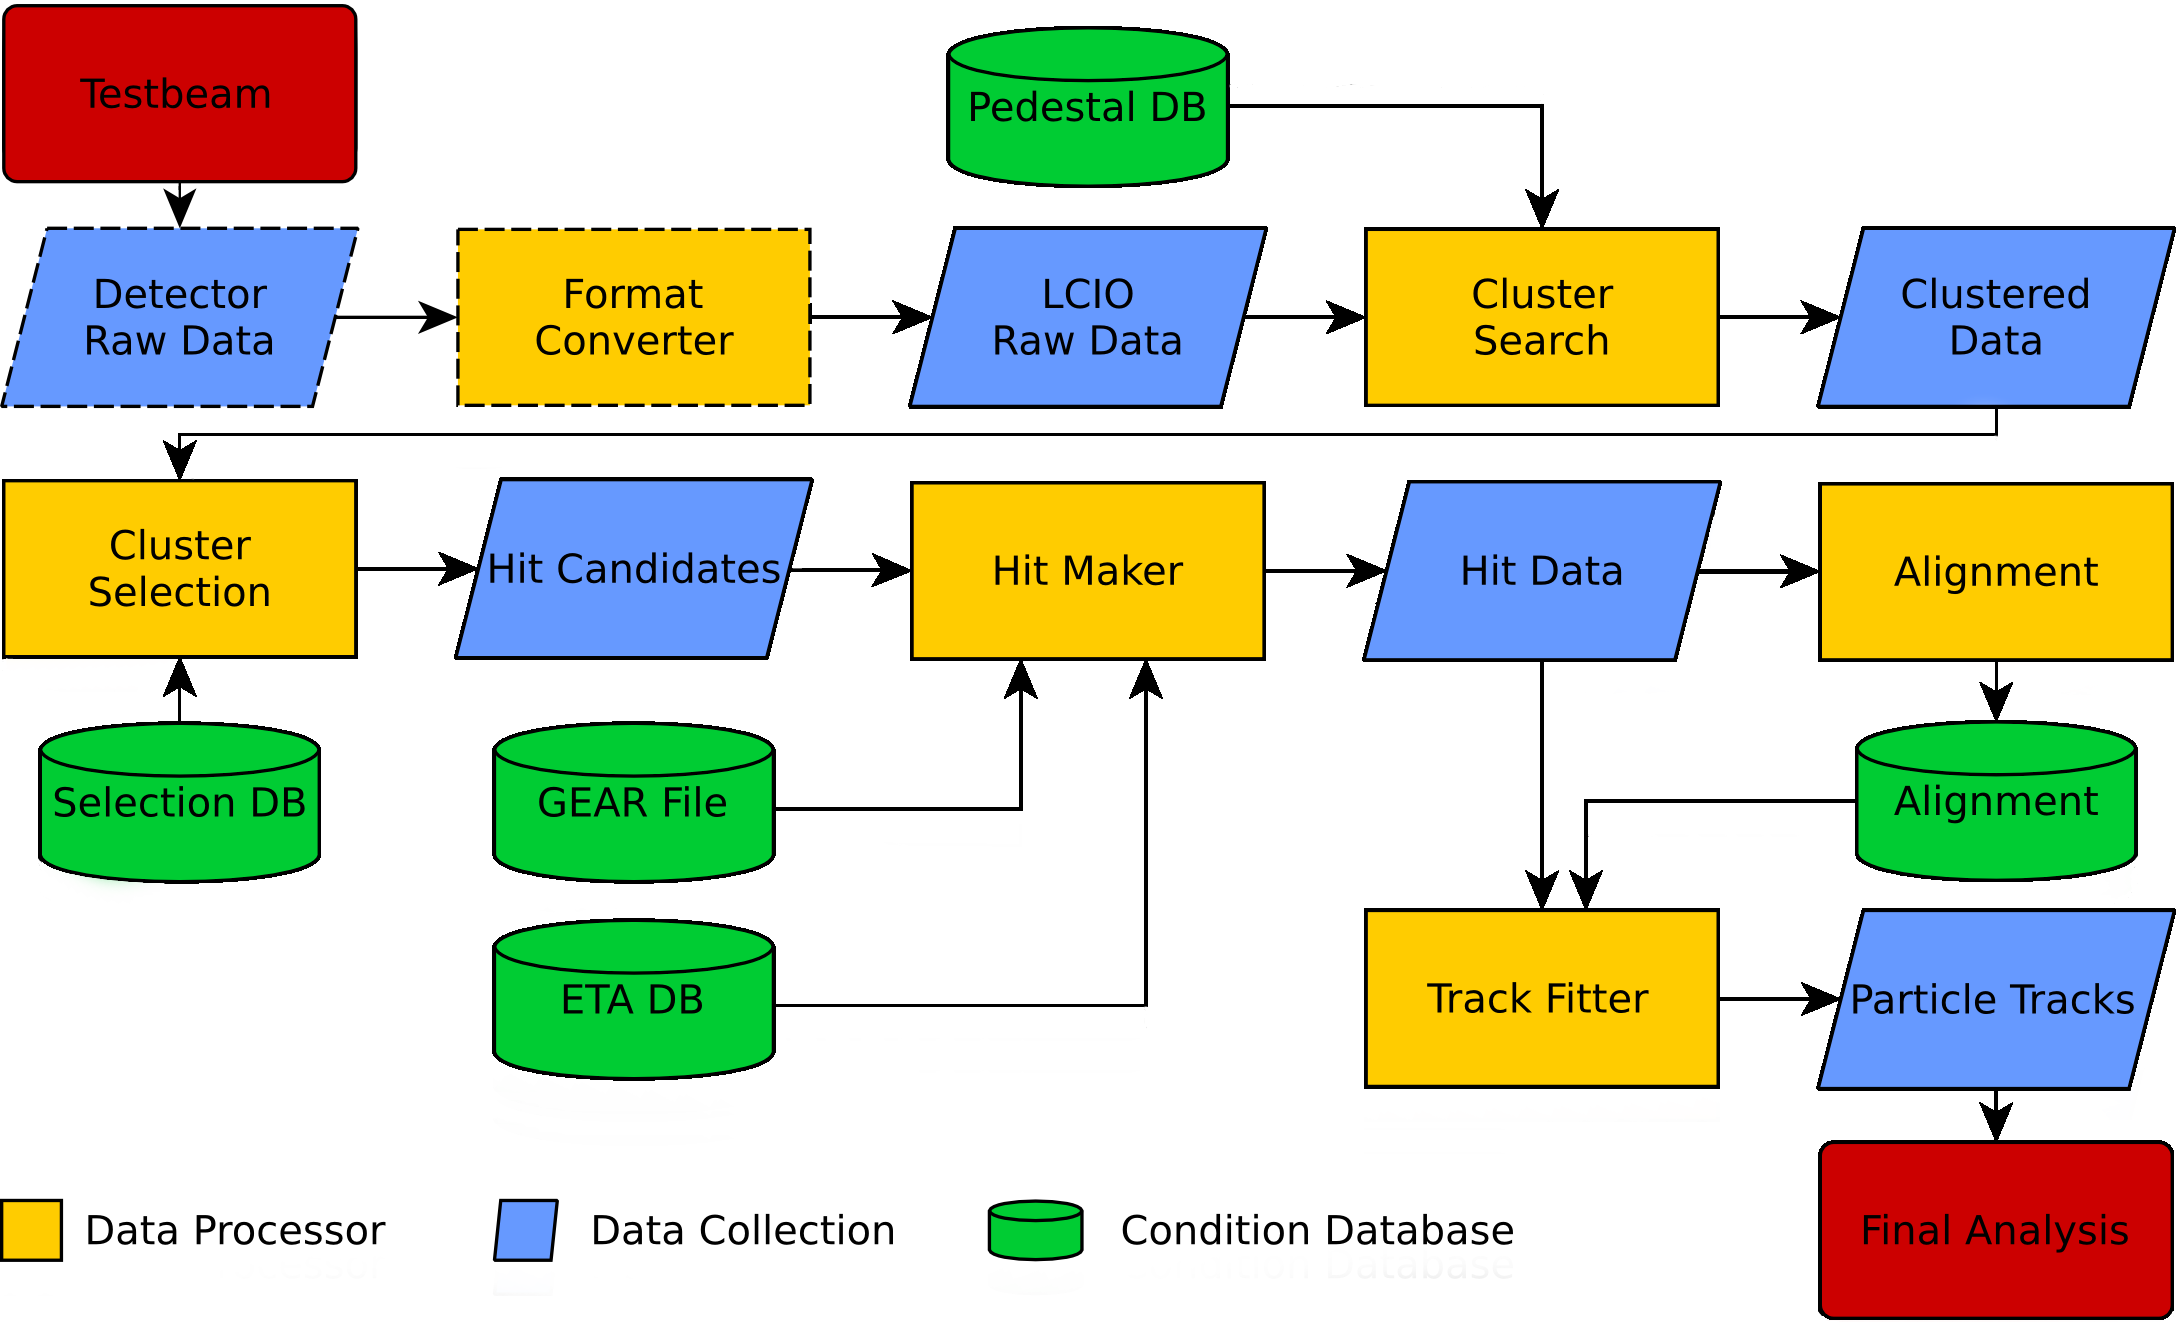
\includegraphics[width=.9\textwidth]{figures/eutel-strategy}
  \caption[The EUTelescope data analysis strategy]{Schematic of the overall telescope data reconstruction and analysis strategy of the EUTelescope framework.
EUTelescope provides processors for all steps, except for the conversion of the DUT raw data, marked with a dashed outline.}
  \label{fig:offline:strategy}
\end{figure}


